\paragraph{Primary comparison.}
Table~\ref{tab:pathtable} reports flow prediction, attribution accuracy,
and the end-to-end error of the reported summary on the same test demand
paths for both networks. On the 96 Sioux Falls paths, response
supervision lowers the median attribution-column error from $21.18\%$ to
$14.19\%$ (a relative reduction of one third) and the family-boundary
error from $8.74\%$ to $5.75\%$, while both models retain total-flow
errors near $0.03\%$ (medians $0.0322\%$ and $0.0292\%$). Measured
against the demand-change increment rather than total flows, the
endpoint flow-prediction error falls from $5.03\%$ to $3.52\%$ --- the
incremental response that the attributions decompose --- so response
supervision improves both the attribution column and the response field
it integrates; the total-flow columns stay near $0.03\%$ because total
flows are dominated by the unchanged background. The improvement holds
in every active-query group
(Appendix~\ref{supp:learningdetail}). Path-level paired differences
quantify the uncertainty: the median paired column-error difference is
$-5.03$ percentage points with a path-level bootstrap $95\%$ interval of
$[-6.01,-4.48]$ (10,000 resamples), improving 92 of 96 paths; the
paired family-boundary difference has median $-2.06$ with interval
$[-2.76,-1.65]$, improving 90 of 96, with every group's interval
excluding zero and leave-one-path-out medians varying within
$[-5.11,-4.94]$ and $[-2.11,-2.00]$. The system-contribution difference
is secondary and opposite in sign (median $+0.45$, interval
$[0.01,0.74]$; both methods below $3.5\%$), confirming that scalar
completeness and spatial explanation accuracy measure different
properties. The improvement is consistent across all five seeds, with
both median error metrics decreasing for every seed and 80--91 of 96
paths improving per seed (Table~\ref{tab:fiveseed},
Appendix~\ref{supp:learningdetail}). The same-path decomposition of
Eq.~\eqref{eq:coldecompmain} attributes the discrepancy to demand-response
error on every path--query pair (path--query median response and weight
norms $206.5$ and $3.5$ under flow supervision, $147.6$ and $3.3$ under
response supervision).
\begin{table}[t]\centering\footnotesize
\caption{Prediction and spatial-explanation accuracy, and the end-to-end
error of the reported summary, on the same test demand paths (Sioux
Falls: 96 paths, 24 per active-query group; Anaheim: 48 paths). Entries
are medians of path-level values (active queries and seeds averaged
within each path; flow errors additionally averaged over the path's
states). Total flow: relative flow error; incremental: endpoint
flow-change error (percent of the reference increment norm); column:
attribution-column error; family boundary: maximum boundary error over
the query's family as a percentage of the reference family maximum (the
Sioux Falls family is the geometric screenline set; Anaheim uses its
ordered distance family); final summary: total error of the reported
minimum-segment summary (percent of the reference family scale;
tolerance $5\%$ of the learned family maximum); Seg./chain: median
segments per ordered direction chain (Anaheim's family is one ordered
chain); total segments: median over all distinct chains (Sioux Falls,
18--35 chains per query) or over the single family (Anaheim) --- the two
networks' totals are not comparable one to one.}\label{tab:pathtable}
\setlength{\tabcolsep}{3.4pt}
\begin{tabular*}{\tblwidth}{@{\extracolsep{\fill}}llccccccc}
\toprule
Network & Method & Total flow (\%) & Incremental (\%) & Column (\%) & Family (\%) & Final summary (\%) & Seg./chain & Total seg.\\
\midrule
Sioux Falls & Flow & 0.032 & 5.03 & 21.18 & 8.74 & 11.35 & 3.6 & 117\\
Sioux Falls & Response & 0.029 & 3.52 & 14.19 & 5.75 & 8.68 & 3.6 & 117\\
\addlinespace
Anaheim & Flow & 0.024 & 2.46 & 1.64 & 0.94 & 4.57 & 9.9 & 9.9\\
Anaheim & Response & 0.019 & 2.03 & 1.31 & 0.78 & 4.55 & 9.9 & 9.9\\
\bottomrule\end{tabular*}\end{table}

\paragraph{Where the flow-only explanation breaks, and what supervision
repairs.}
Figure~\ref{fig:repair} shows one pre-specified case: among the 96 test
paths, the one whose paired family-error improvement is closest to the
median improvement (path 22, six active queries; improvement $48.4$
against the median $49.2$), and within it the query with the largest
flow-only family error, OD $(7,12)$. The panels display the query's
longest projection-direction chain (20 nested boundaries, a geometric
display choice independent of attribution values), the boundary error
against the reference along that chain, and the family-wide worst
boundary on the network. The flow-only model does not merely rescale
the profile: it misplaces the attribution across the corridor, with
errors concentrated where the reference profile varies. At the worst
flow-only boundary ($369.5$ TSTT units, on a reference value of
$5{,}619.3$ that is congestion-dominated: $5{,}018.7$ of it from
congestion weights against $600.6$ from free-flow weights) the error
falls to $80.1$ under response supervision --- a $78\%$ reduction at
that boundary; over the whole family, the worst error falls from
$369.5$ to $115.2$ and the end-to-end error of the reported summary
from $679.1$ to $463.7$ at essentially unchanged segment count ($186$
to $190$ over the family). All quantities come from the same
five-seed-median columns the figure displays. The segment summaries of
all three columns sit inside their stated tolerance bands, so the
repair acts on the profile the summaries compress, not on the
compression itself.
\begin{figure}[t]
\centering
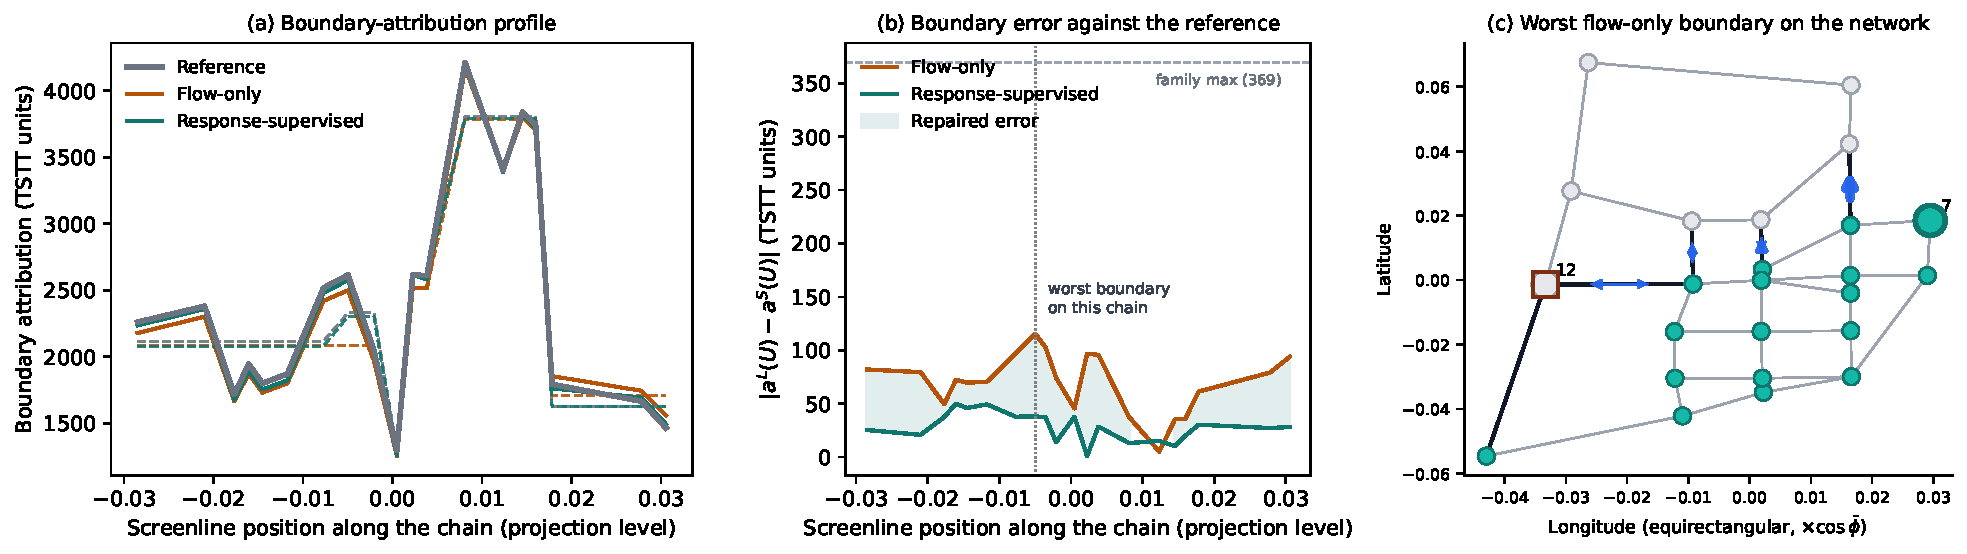
\includegraphics[width=\linewidth]{../figures/fig_v111_repair.pdf}
\caption{A learned spatial profile repaired by response supervision
(pre-specified case: path 22, query $(7,12)$; five-seed median columns).
(a)~Boundary-attribution profile along the query's longest
projection-direction chain (20 nested boundaries at the $10^\circ$
direction): reference (gray), flow-only (ochre), response-supervised
(teal), each with its minimum-segment summary (dashed). (b)~Boundary
error against the reference along the same chain; the dotted line marks
the worst boundary on the chain and the gray dashed line the
family-wide maximum ($369.5$). (c)~The family-wide worst flow-only
boundary on the network: teal nodes form $U$ (origin $7$ ringed,
destination $12$ square); arrow width scales with the signed
crossing-link contribution (solid blue positive, dashed red
negative).}\label{fig:repair}
\end{figure}

\paragraph{The objective family.}
The boundary-error representation of
Eq.~\eqref{eq:localboundarybound} defines a family of supervision
objectives rather than a single loss; the complete six-objective
comparison, including the weighted form identified by
Eq.~\eqref{eq:coldecompmain} and the boundary-seminorm loss, appears
in Appendix~\ref{app:legacy-learning}. Two of its results organize the
present comparison. The unweighted response objective attains the
lowest errors on every metric (column $14.19\%$, family boundary
$5.75\%$, flow $0.029\%$) with the widest usable weight range, while
its weighted form reaches $15.21\%$ --- the weight-shift term the
unweighted objective ignores is small. And $\mathcal K_j$ is a seminorm
whose kernel contains the circulation directions, so optimizing the
boundary value alone cannot restore the response field the profile
integrates: the boundary-seminorm objective attains the lowest
validation boundary error yet a test column error above flow-only
training ($24.18\%$, improving only 8 of 96 paths).

\paragraph{Label efficiency, training budget, and wall-clock.}
The improvement is cheap in labels and stable in budget. Retraining at
per-query derivative-center budgets of 6--48 (36--288 centers; full
budget 384) reaches half of the full column-error improvement at 36
centers and $90\%$ at 288, with subset interquartile ranges below
$0.8$ percentage points and flow accuracy unchanged
(Figure~\ref{fig:v109labelbudget}, Appendix~\ref{app:labelbudget}).
Tripling the continuation budget to 3{,}600 updates improves both
methods on both networks while the response curve stays below the flow
curve at every update count (Figure~\ref{fig:v109convergence},
Appendix~\ref{supp:learningdetail}): the median column error falls to
$19.46\%$ against $11.41\%$ on Sioux Falls and $1.24\%$ against
$0.88\%$ on Anaheim. Derivative supervision costs more per update
($1.8\times$ on Sioux Falls, $3.3\times$ on Anaheim); on Sioux Falls
the anytime dominance survives the cost difference in wall-clock
terms, while on Anaheim the response run reaches the flow method's
final error after about $2.2$ times its training time.

\paragraph{End-to-end explanation error.}
The quantities of Table~\ref{tab:pathtable} concern the learned
profiles; the reported artifact is the learned model's minimum-segment
summary, whose total error Table~\ref{tab:pathtable} already carries as
the budget of Eq.~\eqref{eq:totalbudget} at the working $5\%$ tolerance.
Figure~\ref{fig:v110resolution} traces the same quantities as the
tolerance --- and with it the number of reported segments --- varies
from $0.5\%$ to $10\%$, and Table~\ref{tab:matched} reports the
matched-complexity comparison over that pre-specified grid: at each
tolerance the two methods segment their own learned profiles, and the
paired difference is evaluated at the matched segment budget --- the
smaller of the two methods' per-path segment counts, each method
interpolated on its own error--segments grid.
The two networks occupy different regimes, and the error budget
identifies the effective lever on each. On Sioux Falls the model term
dominates ($8.74\%$ against a $4.76\%$ summary term under flow
supervision), the response-supervised curve lies below the
flow-supervised curve at every segment count: at the matched segment
budget of each tolerance (Table~\ref{tab:matched}) the paired median
difference is $-1.7$ to $-2.0$ percentage points with bootstrap
intervals excluding zero at every tolerance --- computed on all 96
paths' data at $0.5$--$2.5\%$ and on the common-support subset at the
two loosest tolerances, where the equal-tolerance comparison over all
paths is essentially identical (individual paths can still move the
other way; the intervals are for the median) --- and the iso-error view
quantifies the
saving: a final error of $11.0\%$ needs $152$ segments under flow
supervision but $117$ under response supervision, while the $8.8\%$
error that response supervision attains with $117$ segments is not
reached by flow supervision anywhere in the grid (its best, $8.80\%$,
requires $233$ segments). On Anaheim the learned columns are closer to
the reference, and at the working $5\%$ tolerance the budget is
compression-dominated: the summary term ($4.3\%$) is several times the
model term ($0.9\%$), both curves track the reference-compression
curve --- the error of compressing the reference profile itself at each
tolerance --- and the two methods are nearly indistinguishable in the
final error ($4.57$ against $4.55$), exactly as the budget predicts:
the model error is not the active bottleneck there, and tolerance
refinement, not a better learned response, is the effective
intervention. At the tightest $0.5\%$ tolerance the model term takes
over ($0.9\%$ and $0.8\%$ against a $0.5\%$ summary term), where the
response-supervised final error is again lower ($0.91\%$ against
$1.06\%$). Better learned responses matter precisely when model error
is the active bottleneck; when compression dominates, the framework
correctly identifies tolerance refinement as the relevant lever. On
both networks the measured total error of the reported summary stays
within the budget on every path. Relative to the baselines,
segmentation cuts the total error by a factor of $3.0$--$3.8$ (single
common value) and $1.7$--$2.0$ (equal-count) on Sioux Falls, and by
$10.5$--$10.6$ and $10.2$ on Anaheim --- where the strongly ordered
profiles make equal-count segmentation nearly as coarse as a single
value, so position-aware segmentation is what carries the error
control. The final-summary entries of Table~\ref{tab:pathtable} are
medians of budget components computed on each path--query--seed before
aggregation, so they do not add to a guarantee for any single
explanation.

\begin{table}[t]\centering\footnotesize
\caption{Matched-complexity end-to-end comparison over the
pre-specified tolerance grid. At each tolerance both methods segment
their own learned profiles. $L$: median total segment count (Sioux
Falls: distinct chains; Anaheim: single ordered family). Error: median
normalized total error of the reported summary (percent of the
reference family scale, as in Table~\ref{tab:pathtable}). The paired
difference is computed at the matched segment budget
$L^{*}=\min(L_{\mathrm{flow}},L_{\mathrm{response}})$ of each path:
each method is interpolated linearly on its own five-point
(error,~segments) grid, and the median per-path paired difference
(response $-$ flow) receives a path-level bootstrap $95\%$ interval
(5{,}000 resamples). Only paths whose $L^{*}$ lies inside both
methods' grid support are compared ($n$; budgets outside a grid are
excluded, not clamped): all 96 Sioux Falls paths at $0.5$--$2.5\%$,
95 at $5\%$, and 14 at $10\%$, where the two grids barely overlap;
all 48 Anaheim paths except 13 at $10\%$. The equal-tolerance medians
(no interpolation, all paths) differ from the tabulated differences by
at most $0.11$ percentage points and exclude zero at every tolerance
on both networks.}\label{tab:matched}
\setlength{\tabcolsep}{4.2pt}
\begin{tabular*}{\tblwidth}{@{\extracolsep{\fill}}lrrrrrrr}
\toprule
 & \multicolumn{2}{c}{Flow} & \multicolumn{2}{c}{Response} & \multicolumn{3}{c}{Matched-budget difference}\\
\cmidrule(lr){2-3}\cmidrule(lr){4-5}\cmidrule(l){6-8}
Tolerance & $L$ & Error (\%) & $L$ & Error (\%) & $L^{*}$ & $n$ & Median (pp) [$95\%$ interval]\\
\midrule
\multicolumn{8}{l}{\emph{Sioux Falls} (96 paths; model-error dominated)}\\
$0.5\%$ & 233 & 8.80 & 235 & 5.82 & 233 & 96 & $-2.02$ $[-2.70,-1.60]$\\
$1\%$ & 202 & 9.01 & 201 & 6.04 & 201 & 96 & $-1.98$ $[-2.68,-1.64]$\\
$2.5\%$ & 152 & 9.63 & 152 & 6.91 & 152 & 96 & $-1.93$ $[-2.59,-1.49]$\\
$5\%$ & 117 & 11.35 & 117 & 8.68 & 117 & 95 & $-1.68$ $[-2.41,-1.28]$\\
$10\%$ & 77 & 13.93 & 77 & 11.51 & 25 & 14 & $-1.78$ $[-3.06,-1.25]$\\
\addlinespace
\multicolumn{8}{l}{\emph{Anaheim} (48 paths; compression dominated at $5\%$)}\\
$0.5\%$ & 28 & 1.06 & 27 & 0.91 & 27 & 48 & $-0.16$ $[-0.20,-0.08]$\\
$1\%$ & 21 & 1.37 & 21 & 1.24 & 21 & 48 & $-0.11$ $[-0.17,-0.07]$\\
$2.5\%$ & 12 & 2.54 & 12 & 2.49 & 12 & 48 & $-0.06$ $[-0.08,-0.02]$\\
$5\%$ & 10 & 4.57 & 10 & 4.55 & 10 & 48 & $-0.02$ $[-0.04,-0.01]$\\
$10\%$ & 6 & 8.14 & 6 & 8.13 & 6 & 35 & $-0.03$ $[-0.05,-0.01]$\\
\bottomrule\end{tabular*}\end{table}

\paragraph{Beyond the labeled response domain.}
Both the derivative centers and the 96 test paths draw base demands
from $[0.65,1.3]$ times the published OD vector, so the improvement
could be specific to that labeled band. Two out-of-domain bands ---
low loads on $[0.40,0.60]$ and high loads on $[1.35,1.55]$, 24 paths
each under the test generator's rules --- separate the two
extrapolation directions. On the high-load band, adjacent to the
labeled domain, response supervision remains better on every metric
(paired medians: column $-1.31$, family boundary $-0.68$, unrestricted
extrema $-5.30$ percentage points, all intervals excluding zero). On
the low-load band, far from the labeled domain, the advantage
disappears: the family-boundary and summary errors are slightly higher
under response supervision (paired medians $+0.68$ and $+0.57$
percentage points, intervals $[+0.18,+1.06]$ and $[+0.07,+0.90]$),
with the column error statistically indistinguishable ($+1.25$,
$[-0.17,+2.99]$). Response supervision therefore provides its gain
inside and near the labeled response domain and preserves the error
ordering under moderate extrapolation toward higher loads; the low-load
band marks where the labeled derivative information stops
transferring (Appendix~\ref{app:pairs-v102}).
\begin{figure}[t]
\centering
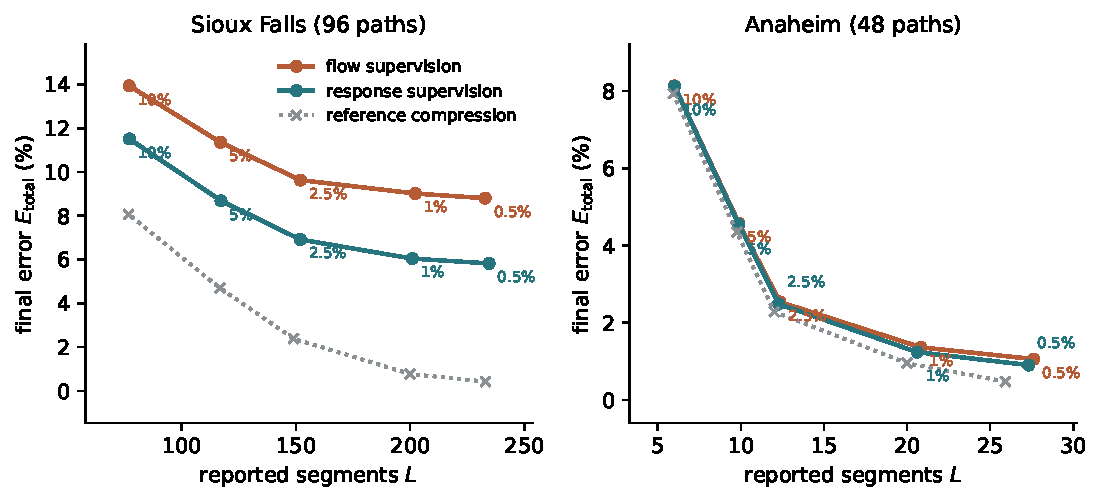
\includegraphics[width=\linewidth]{../figures/fig_v110_resolution.pdf}
\caption{Final error of the reported summary against the number of
reported segments, as the family tolerance varies over $0.5$--$10\%$
(annotated; percent of the learned family maximum). Sioux Falls
(left): model-error dominated --- the response-supervised curve (teal)
lies below the flow-supervised curve (ochre) at every segment count, so
better responses convert into either fewer segments at equal accuracy
or more accurate summaries at equal complexity. Anaheim (right):
compression dominated at the working tolerance --- both curves track
the gray reference-compression curve, the error of compressing the
reference profile itself at each tolerance, plotted at its own segment
count ($\times$ marks). Per-tolerance segmentation recomputed from the
final learned profiles; common per-query normalization as in
Table~\ref{tab:pathtable}.}\label{fig:v110resolution}
\end{figure}

\paragraph{Bound tightness.}
Computed with the same $41$-state trapezoidal quadrature for both
sides, the exact unrestricted errors $\mathcal K_j(e_j)$ lie below the
integrated bounds $B_j$ of Eq.~\eqref{eq:localboundarybound} (the
numerical verification and quadrature accuracy are reported in
Appendix~\ref{supp:accuracy}). The chain is tight: the median ratio
$\mathcal K_j(e_j)/B_j$ is $0.95$ for flow supervision (quartiles
$0.91$--$0.98$) and $0.95$ for response supervision (quartiles
$0.90$--$0.97$). The integrated bound is therefore a tight
\emph{a posteriori} upper bound on the realized worst boundary error
--- it uses reference-response information, as
Section~\ref{sec:totalbudget} notes --- and response supervision lowers
the family, unrestricted and bound levels in parallel. The geometric
family retains about half of the unrestricted error (median ratio
$E^{\mathrm{geo}}/\mathcal K_j(e_j)$ $0.51$ and $0.48$), so the
single-family errors reported throughout should be read as lower
bounds on the worst separating-region error.
